\section{Modelling and Analysis of Master Algorithm}
\label{sec:ma}
The master algorithm (MA) provides the orchestration of FMUs, which denotes the co-simulation of various FMUs. To ensure the correctness of co-simulation execution process, it is necessary to verify certain properties of the master algorithm. In this section, we use timed automata to model three versions of master algorithms and verify some expected properties of master algorithm such as deadlock, liveness and reachability with UPPAAL.
\subsection{I/O Dependency Information}
When it comes to co-simulation, I/O dependency information \cite{BromanBGLMTW13} is inevitably required to be well considered. The master algorithm calls function \emph{Set} to provide input value to an FMU and function \emph{Get} to retrieve an output value. So it is essential to know which outputs of an FMU depend immediately on which inputs. In the design of a MA, the direct dependency information can be used to call the function \emph{Set} and \emph{Get} in a well-defined order. In FMI 2.0, this information can be provided using the element \emph{ModelStructure} \cite{FMI2INTRO}. However, sometime there may be an algebraic loop in the dependency information, which may not converge. Since we are interested in non-diverging and deterministic composition of FMUs, we need to distinguish these two cases. 
\subsection{Master Algorithm}
The master algorithm is to orchestrate the execution of different subsystems. Each subsystems serves as an FMU block whose simulation is triggered by a particular MA. FMUs can be seen as black boxes comprising input. The process of simulation is divided into several steps where each FMU can be simulated independently until it needs to exchange data or implement synchronization. There are three versions of master algorithm,which is shown in Fig.\ref{ad-fixedstep}.
\begin{figure}[htbp]
\centering{
		\subfigure[Fix step size algorithm]{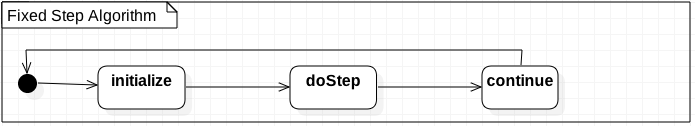
\includegraphics[width=3.5in,height=0.8in]{fig/MA1.png}
			\label{sd_fixedstep}}
		\hfil
		\subfigure[Rollback algorithm]{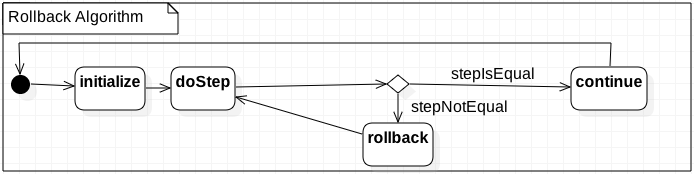
\includegraphics[width=3.5in,height=0.9in]{fig/MA2.png}
			\label{sd-rollback}}	
		\subfigure[Predictable step sizes algorithm]{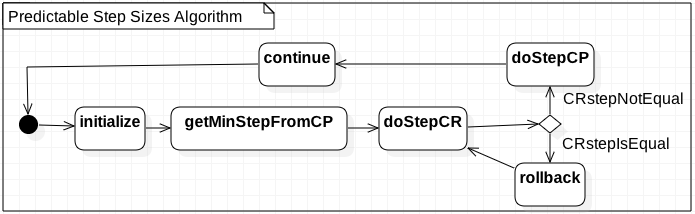
\includegraphics[width=3.5in,height=1.1in]{fig/MA3.png}
			\label{sd-pre}}		
	\caption{Activity diagrams for three versions of master algorithms.}
	\label{ad-fixedstep}
	}
\end{figure}
\subsubsection{Fixed Step Algorithm}
In fixed step algorithm, all FMUs have the same step size. When master algorithm calls \emph{doStep} with the step size \emph{h}, time will advance from a communication point \emph{t} to the next communication point \emph{t+h}. During the simulation step, an FMU with it's own solver will simulate independently according to its input value and generate a running result as output value. MA will wait until all FMUs finish their simulation step and then get their output values to exchange data for preparing next simulation step. The activity diagram of fixed step algorithm is illustrated in Fig.\ref{sd_fixedstep}. There are mainly three activities in the control flow: \emph{initialize}, \emph{doStep} and \emph{continue}. In the fixed step algorithm \cite{BromanBGLMTW13}, the process can maintain correct when all FMUs are reliable. When some error happens during a simulation step, the process will be affected after the wrong simulation step. Then we need the FMU rollback mechanism.
\subsubsection{Rollback Algorithm}
There are some important features proposed in the FMI 2.0. We can save the FMU state if necessary and the state we saved in the process can be restored. For example, MA calls \emph{doStep} on $FMU_{1}$ and $FMU_{2}$ while $FMU_{1}$ can accept the request or $FMU_{2}$ can reject it. If we save the state of $FMU_{1}$ and $FMU_{2}$ at the communicating point \textrm{t}, we can restore the scene after $FMU_{2}$ rejects \emph{doStep}. Under this circumstances, we need all FMUs support rollback. The activity diagram of rollback algorithm is clearly shown in Fig.\ref{sd-rollback}. Compared with the fixed step algorithm, all FMUs are required to support \emph{rollback} mechanism, that is, all FMUs need to return to the previous state if the simulation step sizes of all FMUs are not equal.
\subsubsection{Predictable Step Size Algorithm}
To improve the efficiency of MA, it is important to predict step size. So predictable step size algorithm is proposed. The function \emph{GetMaxStepSize} was introduced to optimize the performance of rollback algorithm. This function return the maximum step size and state flag of a predictable FMU. Maximum step is the largest step that a predictable FMU can perform. State flag includes \emph{ok}, \emph{discard} and \emph{error}. \emph{OK} denotes the predictable FMU can accept the simulation step size. \emph{Discard} denotes the predictable FMU only implement partial step during simulation. \emph{Error} denotes the predictable FMU can't continue the simulation because of its unacceptable state or unreasonable input value. Also, when \emph{discard} and \emph{error} happen, the FMU need to rollback to the previous state saved before. Whether an FMU is a predictable FMU or not should be indicated in FMU's \emph{xml} file. Moreover, if an FMU supports rollback and predictable step size at the same time, the predictable step size algorithm only uses predictable ability to get the maximum step of a predictable FMU. On the other hand, a predictable FMU can accept any step size less than or equal to the maximum step returned by \emph{GetMaxStepSize}.

First, the master algorithm chooses the maximum step size of all predictable FMUs and find the smallest communication step size \emph{h} that all predictable step size can be accepted. Then, we save the states of all FMUs. MA calls \emph{doStep(h)} on FMUs supporting rollback. The function \emph{doStep()} will return the real performed step size. If all performed step sizes are equal to \emph{h}, MA will call \emph{doStep(h)} on FMUs. Otherwise, MA will find the smallest performed step $h_{min}$, then all FMUs will restore the state saved before the co-simulation. Finally, MA will invoke $doStep(h_{min})$ on all FMUs. The control flow of predictable step size algorithm is shown in Fig.\ref{sd-pre}. For example, \emph{getMinStepFromCP} is an activity that MA will call \emph{GetMaxStepSize} on all predictable FMUs to find their maximum simulation step size and then return the smallest one of them. 

\subsection{Modelling and Analysis of MA} 
To verify the correctness of three versions of master algorithms, we model the master algorithms using timed automata in UPPAAL. The following Fig.\ref{ta-master} shows the execution of three master algorithms in the form of timed automata respectively. Fixed step algorithm has \emph{Init}, \emph{doStep} states and synchronize with FMU by channel \emph{continue}. Rollback algorithm has \emph{Init}, \emph{DoStep}, and \emph{Continue} states. If all FMUs don't have the same step size, rollback algorithm will communicate with FMUs by \emph{rollback} signal, otherwise, it will send \emph{continue} signal and move to \emph{Continue} state. Predictable step size algorithm has \emph{Init}, $find \_ CP \_ MIN$, \emph{DoStep}, \emph{writeCP} states. It obtains the minimal step size (i.e., \emph{step2}) of FMUs supporting \emph{GetMaxStepSize} function and the maximal step size (i.e., \emph{step1}) of FMUs supporting rollback function. If \emph{step1} is greater than \emph{step2}, FMUs receive \emph{rollback} signal and return to \emph{DoStep} state. Otherwise, FMUs receive \emph{continue} signal and do the next step.  



\begin{figure}[htbp]
\centering{
		\subfigure[Timed automata for fixed step algorithm]{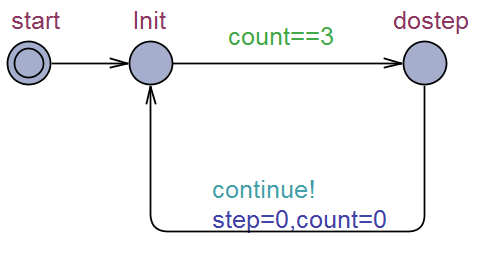
\includegraphics[width=1.0in,height=0.8in]{fig/fixedstep_master.png}
			\label{ta_fixedstep}}
		\hfil
		\subfigure[Timed automata for rollback algorithm]{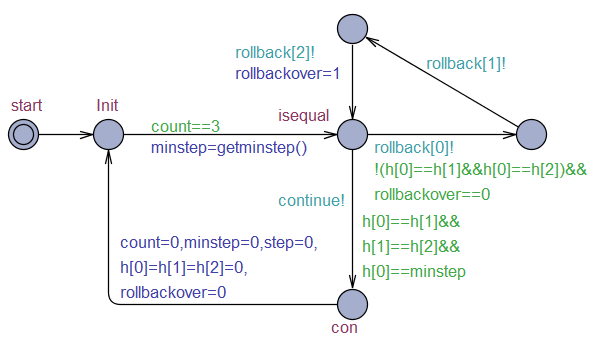
\includegraphics[width=2.0in,height=1.2in]{fig/rollback_master.png}
			\label{ta-rollback}}	
		\subfigure[Timed automata for predictable step sizes algorithm]{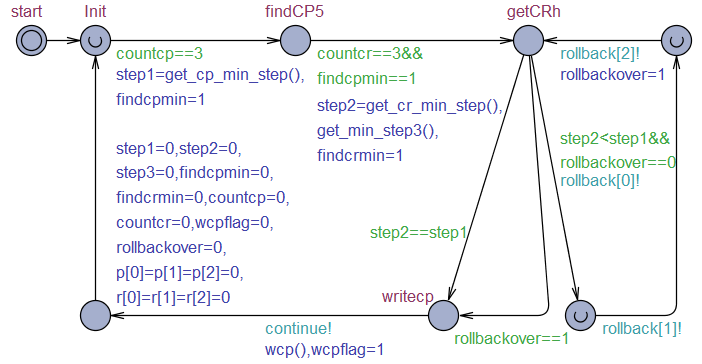
\includegraphics[width=3.5in,height=1.6in]{fig/pma_master.png}
			\label{ta-pre}}		
	\caption{Timed automata for three version of master algorithms.}
	\label{ta-master}
	}
\end{figure}


 
We verify the properties of master algorithms including reachability, liveness and deadlock. Experimental results are shown in Table \ref{rs}, where:

\begin{itemize}
\item
$E \langle\rangle ~master.dostep$, $E\langle\rangle~master.Continue$ and $E\langle\rangle~master.writecp$ are reachability properties checking whether the model can reach these states;
\item
$master.Init \rightarrow master.dostep$, $master.Init \rightarrow master.Continue$ and $master.Init \rightarrow master.Continue$ are liveness property. If the master algorithm arrives at former state, it eventually reaches the latter state;
\item
$A[]~not~deadlock$ is safety property, it means whether the model will be deadlock.
\end{itemize}

In Table \ref{rs}, we can find that the properties such as deadlock, liveness and reachability are satisfied,  which proves the correctness of three master algorithms. For an example, $A[]~not~deadlock$ is satisfied, which means that the execution of the master algorithm will not be deadlock. $master.Init \rightarrow master.doStep$ is satisfied, which means that if the model reach the former state $Init$, it will eventually reach the state $doStep$. $E\langle\rangle~master.doStep$ is satisfied, which means that there exists a reachable state $doStep$. 

\begin{table}
\caption{Checking Properties of Master Algorithms}
\centering
\begin{tabular}{c c c}
        \hline
        MA & Property & Result\\
        \hline
        \multirow{2}{2.0cm}{Fixed Step}
                & $A[]~not~deadlock$ & True\\
                & $master.Init \rightarrow master.dostep$ & True\\
                & $E\langle\rangle~master.dostep$ & True\\

        \hline
        \multirow{2}{2.0cm}{Rollback}
                & $A[]~not~deadlock$ & True\\
                & $master.Init \rightarrow master.Continue$ & True\\
                & $E\langle\rangle~master.Continue$ & True\\

        \hline
        \multirow{2}{2.0cm}{Predictable}
                & $A[]~not~deadlock$ & True\\
                & $master.Init \rightarrow  master.writeCP$ & True\\
                & $E\langle\rangle~master.writeCP$ & True\\
        \hline
\end{tabular}
\label{ta_rs}
\end{table}

